\documentclass[aspectratio=169,12pt,t]{beamer}

% --- Theme: Metropolis (modern, clean) ---
\usetheme[progressbar=frametitle,numbering=fraction,block=fill]{metropolis}

% --- Fira Sans font (install texlive-fonts-extra if missing) ---
\IfFileExists{FiraSans.sty}{\usepackage[sfdefault]{FiraSans}}{}

% --- Light background with warm accent ---
\definecolor{mDarkTeal}{RGB}{35,55,59}
\definecolor{mLightBrown}{RGB}{235,228,216}
\definecolor{mAccent}{RGB}{140,70,20}

\setbeamercolor{normal text}{fg=mDarkTeal,bg=white}
\setbeamercolor{alerted text}{fg=mAccent}
\setbeamercolor{frametitle}{bg=mDarkTeal,fg=white}
\setbeamercolor{progress bar}{fg=mAccent,bg=mLightBrown}
\setbeamercolor{title separator}{fg=mAccent}
\setbeamercolor{progress bar in head/foot}{fg=mAccent,bg=mLightBrown}
\setbeamercolor{progress bar in section page}{fg=mAccent,bg=mLightBrown}

% --- Packages ---
\usepackage[utf8]{inputenc}
\usepackage{amsmath,amssymb,amsthm}
\usepackage{mathrsfs}
\usepackage{tikz}
\usetikzlibrary{arrows.meta,positioning,calc,decorations.pathreplacing,shapes,patterns}
\usepackage{pgfplots}
\pgfplotsset{compat=1.18}

% --- Custom colors for content types ---
\definecolor{defcolor}{RGB}{25,85,120}
\definecolor{thmcolor}{RGB}{140,35,35}
\definecolor{proofcolor}{RGB}{35,100,50}
\definecolor{excolor}{RGB}{140,75,10}
\definecolor{remcolor}{RGB}{90,90,90}

% --- Beamer blocks for mathematical content types ---
\newenvironment{defblock}[1]{%
  \setbeamercolor{block title}{bg=defcolor,fg=white}%
  \setbeamercolor{block body}{bg=defcolor!5}%
  \begin{block}{#1}}{\end{block}}

\newenvironment{thmblock}[1]{%
  \setbeamercolor{block title}{bg=thmcolor,fg=white}%
  \setbeamercolor{block body}{bg=thmcolor!5}%
  \begin{block}{#1}}{\end{block}}

\newenvironment{proofblock}[1]{%
  \setbeamercolor{block title}{bg=proofcolor,fg=white}%
  \setbeamercolor{block body}{bg=proofcolor!5}%
  \begin{block}{#1}}{\end{block}}

\newenvironment{exblock}[1]{%
  \setbeamercolor{block title}{bg=excolor,fg=white}%
  \setbeamercolor{block body}{bg=excolor!5}%
  \begin{block}{#1}}{\end{block}}

\newenvironment{remblock}[1]{%
  \setbeamercolor{block title}{bg=remcolor,fg=white}%
  \setbeamercolor{block body}{bg=remcolor!5}%
  \begin{block}{#1}}{\end{block}}

% --- Metadata ---
\title{Chapter 2: Basic Topology}
\subtitle{Section: Compact Sets}
\author{Based on Walter Rudin's \emph{Principles of Mathematical Analysis}}
\date{}

\begin{document}

% =============================================================================
\begin{frame}
  \titlepage
  \note{
    Welcome back to Chapter 2 of Principles of Mathematical Analysis. In this
    section we study compact sets, which encode a powerful finiteness condition
    that has far-reaching consequences throughout analysis. Compactness is one
    of the most important and subtle concepts in the entire book. It generalizes
    the idea of a closed and bounded subset of the real line to any metric space,
    and it is the right abstraction for many theorems about continuous functions
    and convergence.
  }
\end{frame}

% =============================================================================
\begin{frame}{Outline}
  \tableofcontents
  \note{
    Here is our roadmap. We begin with the definitions of open cover and compact set. Next, a perhaps surprising fact: compactness is intrinsic to the set, unlike openness or closedness. We then connect compactness to closedness and prove a pair of basic preservation theorems. After that we develop the finite intersection property, study nested intervals and nested "k"-cells, and use those tools to prove the climax of the section: every "k"-cell in Euclidean space is compact. Finally, the Heine-Borel theorem and the Bolzano-Weierstrass theorem fall out as one-line corollaries.
  }
\end{frame}

% =============================================================================
% --- Motivation: Why Compactness ---
% =============================================================================

% --- Build 1/3 ---
\begin{frame}{Why Compactness Matters}
  \begin{itemize}
    \item Compactness is a \alert{finiteness condition} on infinite sets
  \end{itemize}
  \note{
    Before we dive into the formal definitions, let us think about what
    compactness is supposed to capture. In one phrase, compactness is a
    finiteness condition. It takes a set that may be infinite and guarantees
    that in some important sense it behaves as if it were finite. This
    is the central intuition to carry with us.
  }
\end{frame}

% --- Build 2/3 ---
\begin{frame}{Why Compactness Matters}
  \begin{itemize}
    \item Compactness is a \alert{finiteness condition} on infinite sets
    \item It generalizes ``closed and bounded'' from $\mathbb{R}$ to metric spaces
  \end{itemize}
  \note{
    On the real line, the sets that behave best under limits and continuous
    functions are the closed and bounded intervals. Compactness is the right
    generalization of this notion to arbitrary metric spaces. In fact, in
    Euclidean space the two notions coincide, a result we will prove as
    the Heine-Borel theorem.
  }
\end{frame}

% --- Build 3/3 ---
\begin{frame}{Why Compactness Matters}
  \begin{itemize}
    \item Compactness is a \alert{finiteness condition} on infinite sets
    \item It generalizes ``closed and bounded'' from $\mathbb{R}$ to metric spaces
    \item It is the right hypothesis for continuity theorems (Chap.~4)
  \end{itemize}
  \note{
    Compactness is the essential hypothesis under which continuous functions
    behave nicely. For instance, a continuous function on a compact set
    attains its maximum and minimum, and is uniformly continuous. We will
    see all of this in Chapter 4. For now, we focus on the topological
    definition and its consequences.
  }
\end{frame}

% =============================================================================
\section{Definitions}
% =============================================================================

% =============================================================================
% --- 2.31 Definition: Open Cover ---
% =============================================================================

\begin{frame}{Definition 2.31: Open Cover}
  \begin{defblock}{Definition 2.31}
    An \alert{open cover} of a set $E$ in a metric space $X$ is a collection
    $\{G_\alpha\}$ of open subsets of $X$ such that
    \[
      E \subset \bigcup_\alpha G_\alpha.
    \]
  \end{defblock}

  \vspace{0.5em}
  \textbf{Key idea:} The open sets $G_\alpha$ together ``cover'' every point of $E$.

  \note{
    Let us start with the idea of an open cover. We have some set "E" sitting
    inside a metric space "X", and we have a collection of open sets, possibly
    infinite or even uncountable, indexed by a parameter alpha. To call this
    collection an open cover of "E", every point of "E" must lie in at least
    one of the open sets. That is all an open cover is. The key word is
    open, which means we are thinking of the sets as neighborhoods that
    surround the points of "E".
  }
\end{frame}

% --- Diagram: Open Cover ---
\begin{frame}{Visualizing an Open Cover}
  \begin{center}
  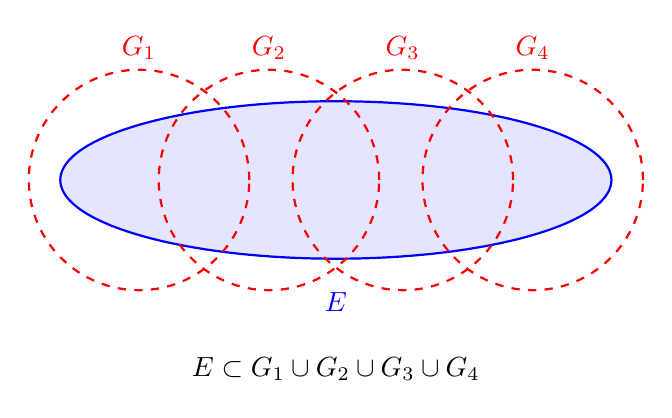
\begin{tikzpicture}[scale=1.0]
    % Set E
    \draw[thick, blue, fill=blue!10] (0,0) ellipse (3.5 and 1);
    \node[blue] at (0,-1.55) {$E$};

    % Covering open sets (radii 1.4; union covers E)
    \draw[thick, red, dashed] (-2.5,0) circle (1.4);
    \node[red, above] at (-2.5,1.4) {$G_1$};

    \draw[thick, red, dashed] (-0.85,0) circle (1.4);
    \node[red, above] at (-0.85,1.4) {$G_2$};

    \draw[thick, red, dashed] (0.85,0) circle (1.4);
    \node[red, above] at (0.85,1.4) {$G_3$};

    \draw[thick, red, dashed] (2.5,0) circle (1.4);
    \node[red, above] at (2.5,1.4) {$G_4$};

    \node at (0,-2.4) {$\displaystyle E \subset G_1 \cup G_2 \cup G_3 \cup G_4$};
  \end{tikzpicture}
  \end{center}

  \note{
    In the picture, the blue region is our set "E", and the four red dashed circles are open sets "G" sub 1 through "G" sub 4. Every point of "E" lies in at least one circle, so their union, shown in the equation below, contains "E". That is what makes this a cover. The picture is a little misleading in one way, though: we only drew four cover elements, but the definition allows arbitrary collections, possibly uncountable. The collection of all open balls of radius one centered at every point of "E" is already an open cover, and it is enormous. The remarkable thing about compactness, which we define next, is that no matter how extravagant the cover, we can always trim it down to finitely many sets.
  }
\end{frame}

% =============================================================================
% --- 2.32 Definition: Compact ---
% =============================================================================

% --- Build 1/2 ---
\begin{frame}{Definition 2.32: Compact Set}
  \begin{defblock}{Definition 2.32}
    A subset $K$ of a metric space $X$ is \alert{compact} if every open cover of $K$
    contains a \alert{finite} subcover.
  \end{defblock}

  \note{
    Here is the central definition of this section. A set is called compact
    if every open cover of it contains a finite subcover. Read this carefully.
    You are handed an open cover, which may be enormous, and you must be able
    to throw away all but finitely many of the sets in it and still cover "K".
    This must work for every open cover, no matter how wild.
  }
\end{frame}

% --- Build 2/2 ---
\begin{frame}{Definition 2.32: Compact Set}
  \begin{defblock}{Definition 2.32}
    A subset $K$ of a metric space $X$ is \alert{compact} if every open cover of $K$
    contains a \alert{finite} subcover.
  \end{defblock}

  \vspace{0.5em}
  More explicitly: if $\{G_\alpha\}$ is an open cover of $K$, then there are
  finitely many indices $\alpha_1, \dots, \alpha_n$ such that
  \[
    K \subset G_{\alpha_1} \cup \cdots \cup G_{\alpha_n}.
  \]

  \note{
    Here is the definition spelled out. Given any open cover "G" sub alpha of "K", compactness guarantees that finitely many indices, alpha one through alpha "n", suffice: the corresponding open sets still cover "K". The word "every" in the previous slide is where the strength lives. It is easy to find some finite cover of almost any reasonable set, but compactness demands a universal statement: any open cover, no matter how cleverly constructed to defeat finiteness, must give in. This is why most proofs invoking compactness work backwards, by exhibiting an awkward open cover that fails to admit a finite subcover and deriving a contradiction. Watch for this pattern in nearly every theorem of this section.
  }
\end{frame}

% --- Remark on compactness ---
\begin{frame}{Remarks on Compactness}
  \begin{remblock}{Remarks}
    \begin{itemize}
      \item Every \emph{finite} set is trivially compact.
      \item Infinite compact sets in $\mathbb{R}^k$ exist (Theorem 2.41).
      \item Compactness is fundamental for continuity (Chap.~4).
    \end{itemize}
  \end{remblock}

  \note{
    A few remarks are in order. First, any finite set is trivially compact:
    just pick one open set from the cover for each of its finitely many
    points. Second, infinite compact sets do exist and in fact abound in
    Euclidean space, as we will prove later. Third, compactness is the
    key hypothesis in many theorems about continuous functions. We will
    see that in Chapter 4.
  }
\end{frame}

% =============================================================================
\section{Compactness Is Intrinsic}
% =============================================================================

% =============================================================================
% --- 2.33 Theorem: Compactness is intrinsic ---
% =============================================================================

\begin{frame}{Theorem 2.33: Compactness Is Intrinsic}
  \begin{thmblock}{Theorem 2.33}
    Suppose $K \subset Y \subset X$. Then $K$ is compact relative to $X$
    if and only if $K$ is compact relative to $Y$.
  \end{thmblock}

  \vspace{0.5em}
  \textbf{Key idea:} Unlike ``open'' or ``closed,'' compactness does \alert{not} depend
  on the ambient metric space.

  \note{
    This theorem says something subtle and important. Recall that whether a
    set is open or closed depends on the surrounding metric space. For example,
    the interval from zero to one is open in itself but not in the real line.
    Compactness, however, is different. Whether a set is compact depends only
    on the set itself, not on any ambient space we happen to embed it in.
    Because of this, it makes sense to speak of a compact metric space in
    isolation, while we never speak of an open space or a closed space
    in the same way.
  }
\end{frame}

% --- Proof Strategy ---
\begin{frame}{Proof Strategy: Theorem 2.33}
  \textbf{Goal:} Show compactness relative to $X$ $\iff$ compactness relative to $Y$.

  \vspace{1em}
  \textbf{Key tool:} Theorem 2.30 --- open sets of $Y$ are exactly
  $V_\alpha = Y \cap G_\alpha$ where $G_\alpha$ is open in $X$.

  \vspace{0.5em}
  \textbf{Approach:}
  \begin{itemize}
    \item ($\Rightarrow$) Given a $Y$-open cover, lift to an $X$-open cover.
    \item ($\Leftarrow$) Given an $X$-open cover, restrict to $Y$.
  \end{itemize}

  \note{
    Before we do the proof, let us understand the strategy. The proof is two
    directions. We use Theorem 2.30 from the previous section, which
    characterizes the open sets of a subspace: a set is open in "Y" if and
    only if it is the intersection of "Y" with an open set of "X". The two
    directions of the proof simply translate open covers back and forth
    using this characterization.
  }
\end{frame}

% --- Proof part 1: Step 1 ---
\begin{frame}{Proof of Theorem 2.33 --- Part 1: $X$ compact $\Rightarrow$ $Y$ compact}
  \begin{proofblock}{Step 1: Lift the cover}
    Let $\{V_\alpha\}$ be open in $Y$ with $K \subset \bigcup_\alpha V_\alpha$.
    By Theorem 2.30, there exist $G_\alpha$ open in $X$ such that
    \[
      V_\alpha = Y \cap G_\alpha.
    \]
  \end{proofblock}

  \note{
    Assume "K" is compact relative to "X". We want to show it is compact
    relative to "Y". Take any open cover of "K" by "Y"-open sets, which we
    call "V" sub alpha. By Theorem 2.30, each "V" sub alpha can be written
    as the intersection of "Y" with some "X"-open set "G" sub alpha. So we
    have lifted the "Y"-open cover to a collection of "X"-open sets. Next,
    we apply compactness in "X".
  }
\end{frame}

% --- Proof part 1: Step 2 ---
\begin{frame}{Proof of Theorem 2.33 --- Part 1: $X$ compact $\Rightarrow$ $Y$ compact}
  \begin{proofblock}{Step 2: Apply $X$-compactness}
    Since $K \subset Y \subset \bigcup_\alpha G_\alpha$ and $K$ is compact in $X$:
    \[
      K \subset G_{\alpha_1} \cup \cdots \cup G_{\alpha_n}. \tag{22}
    \]
    Since $K \subset Y$, intersecting with $Y$ gives:
    \[
      K \subset V_{\alpha_1} \cup \cdots \cup V_{\alpha_n}. \tag{23}
    \]
  \end{proofblock}

  \note{
    Now we apply compactness in "X". Since "K" is contained in "Y", which is contained in the union of the "G" sub alpha, the "G" sub alpha form an "X"-open cover of "K". Compactness in "X" extracts a finite subcover, as shown in equation 22. Then we intersect both sides with "Y". Because "K" already sits in "Y", intersecting with "Y" loses nothing of "K", but it converts each "G" back into the corresponding "V", giving equation 23. So we lifted the cover up to do real work in "X", then descended to recover a clean "Y"-level finite subcover. This pull-up-then-push-down pattern is everywhere in subspace arguments.
  }
\end{frame}

% --- Proof part 2 ---
\begin{frame}{Proof of Theorem 2.33 --- Part 2: $Y$ compact $\Rightarrow$ $X$ compact}
  \begin{proofblock}{Reverse direction}
    Let $\{G_\alpha\}$ be open in $X$ covering $K$. Put $V_\alpha = Y \cap G_\alpha$.
    \begin{itemize}
      \item Each $V_\alpha$ is open in $Y$, and $\{V_\alpha\}$ covers $K$.
      \item By $Y$-compactness: $K \subset V_{\alpha_1} \cup \cdots \cup V_{\alpha_n}$.
      \item Since $V_\alpha \subset G_\alpha$: $K \subset G_{\alpha_1} \cup \cdots \cup G_{\alpha_n}$. \qed
    \end{itemize}
  \end{proofblock}

  \note{
    The reverse direction is the mirror image. This time we start with an "X"-open cover of "K", and we define "V" sub alpha as the intersection of "Y" with "G" sub alpha. By Theorem 2.30 again, each "V" sub alpha is open in "Y", and together they cover "K" because "K" is contained in "Y". Now "Y"-compactness gives us finitely many "V" sub alpha that cover "K", and since each "V" sub alpha is a subset of the corresponding "G" sub alpha, those same "G" sub alpha cover "K". The take-home message is that compactness depends only on which finite subsets of indices witness a cover, not on the ambient space. That is the precise sense in which compactness is intrinsic. Contrast this with openness or closedness, where the very same set can flip status depending on what space we view it inside.
  }
\end{frame}

% =============================================================================
\section{Compactness and Closedness}
% =============================================================================

% =============================================================================
% --- 2.34 Theorem: Compact subsets are closed ---
% =============================================================================

\begin{frame}{Theorem 2.34: Compact $\Rightarrow$ Closed}
  \begin{thmblock}{Theorem 2.34}
    Compact subsets of metric spaces are closed.
  \end{thmblock}

  \vspace{0.5em}
  \textbf{Strategy:} Show the complement $K^c$ is open by proving that every
  point outside $K$ is an interior point of $K^c$.

  \note{
    This is our first real theorem connecting compactness to a familiar
    topological notion. A compact set in any metric space is closed.
    The strategy is standard: to show "K" is closed, we show its complement
    is open by exhibiting a neighborhood of each point outside "K" that
    stays outside "K". The clever part is how compactness comes in.
  }
\end{frame}

% --- Proof Setup ---
\begin{frame}{Proof of Theorem 2.34 --- Setup}
  \begin{proofblock}{Setup}
    Let $K$ be compact and fix $p \in X$, $p \notin K$.

    \vspace{0.5em}
    For each $q \in K$, let $V_q, W_q$ be neighborhoods of $p, q$ of radius
    less than $\tfrac{1}{2} d(p, q)$.
  \end{proofblock}

  \vspace{0.3em}
  \begin{itemize}
    \item $V_q \cap W_q = \varnothing$ (disjoint, by construction).
    \item $\{W_q\}_{q \in K}$ is an open cover of $K$.
  \end{itemize}

  \note{
    We take a point "p" not in "K" and we want to build a neighborhood of "p"
    that avoids "K". The trick is to separate "p" from each point "q" of
    "K" using two disjoint neighborhoods. Since "p" and "q" are distinct,
    their distance is positive, and we use radii less than half that
    distance. The triangle inequality then guarantees the two neighborhoods
    do not meet. Taking all these "W" sub "q" gives an open cover of "K".
  }
\end{frame}

% --- Proof Finish ---
\begin{frame}{Proof of Theorem 2.34 --- Finish}
  \begin{proofblock}{Apply compactness}
    By compactness, finitely many points $q_1, \dots, q_n \in K$ satisfy:
    \[
      K \subset W_{q_1} \cup \cdots \cup W_{q_n} = W.
    \]
    Let $V = V_{q_1} \cap \cdots \cap V_{q_n}$.
    \begin{itemize}
      \item $V$ is a neighborhood of $p$ (finite intersection).
      \item $V \cap W = \varnothing$, so $V \subset K^c$.
    \end{itemize}
    Hence $p$ is interior to $K^c$. \qed
  \end{proofblock}

  \note{
    Now compactness strikes. From the cover of "K" by the "W" sub "q", we
    extract a finite subcover. The corresponding "V" sub "q" are finitely
    many neighborhoods of "p", and we take their intersection, which is
    still a neighborhood of "p" because the intersection is finite. This
    intersection is disjoint from the union of the "W" sub "q", hence
    disjoint from "K". So "p" is in the interior of the complement of "K",
    and we are done. Notice how finiteness was essential for taking an
    intersection of neighborhoods and still getting a neighborhood.
  }
\end{frame}

% --- Diagram: Separation ---
\begin{frame}{Visualizing the Separation}
  \begin{center}
  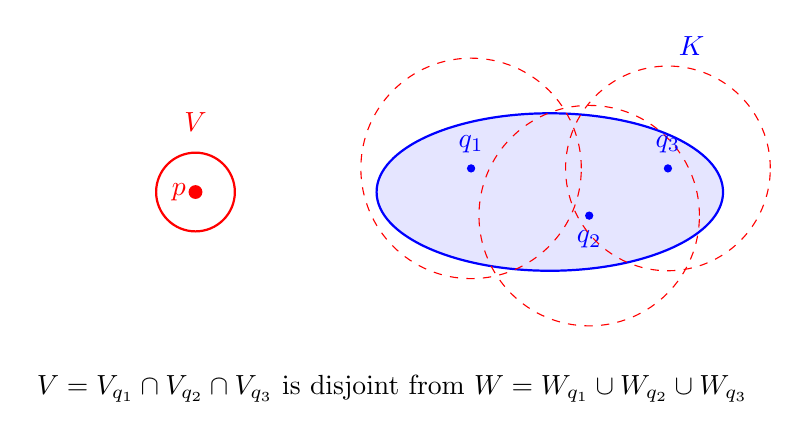
\begin{tikzpicture}[scale=1.0]
    % Compact set K
    \draw[thick, blue, fill=blue!10] (2,0) ellipse (2.2 and 1);
    \node[blue] at (3.8,1.85) {$K$};

    % Point p
    \fill[red] (-2.5,0) circle (2.5pt) node[left]{$p$};

    % q_i points in K and W_{q_i} balls (radii chosen so their union covers K)
    \fill[blue] (1,0.3) circle (1.5pt) node[above=2pt]{$q_1$};
    \draw[red, dashed] (1,0.3) circle (1.4);

    \fill[blue] (2.5,-0.3) circle (1.5pt) node[below=2pt]{$q_2$};
    \draw[red, dashed] (2.5,-0.3) circle (1.4);

    \fill[blue] (3.5,0.3) circle (1.5pt) node[above=2pt]{$q_3$};
    \draw[red, dashed] (3.5,0.3) circle (1.3);

    % V neighborhood of p
    \draw[thick, red] (-2.5,0) circle (0.5);
    \node[red, above=4pt] at (-2.5,0.5) {$V$};

    \node at (0,-2.5) {$V = V_{q_1} \cap V_{q_2} \cap V_{q_3}$ is disjoint from $W = W_{q_1} \cup W_{q_2} \cup W_{q_3}$};
  \end{tikzpicture}
  \end{center}

  \note{
    Here is the setup visualized. The blue ellipse is our compact set "K", and the red dot "p" is an outside point we want to separate. Around each "q" in "K" we draw a red dashed ball "W" sub "q", and we pick a smaller ball "V" sub "q" around "p" so that the two are disjoint. The diagram shows three representative "q" points with their "W" balls; together those balls cover "K". By compactness, we only need finitely many, three in the picture, to still cover. The solid red ball around "p", labeled "V", is the intersection of the corresponding "V" sub "q", and it avoids all three "W" balls, hence avoids "K". Notice what compactness is really doing here. Each pair of balls separates just two points, "p" from one "q". With infinitely many "q" inside "K", intersecting all the corresponding balls around "p" could collapse to a single point, leaving no neighborhood at all. Compactness reduces the problem to finitely many "q", and a finite intersection of open balls is still an open ball. This finite-versus-infinite distinction is the entire engine of the proof, and the reason "K" had to be compact in the first place.
  }
\end{frame}

% =============================================================================
% --- 2.35 Theorem: Closed subsets of compact are compact ---
% =============================================================================

\begin{frame}{Theorem 2.35: Closed Subsets of Compact Sets Are Compact}
  \begin{thmblock}{Theorem 2.35}
    Closed subsets of compact sets are compact.
  \end{thmblock}

  \vspace{0.5em}
  \textbf{Strategy:} Given an open cover of $F$, add $F^c$ to get an
  open cover of $K$, extract a finite subcover, and discard $F^c$.

  \note{
    This is a nice companion to Theorem 2.34. If "F" is closed and sits
    inside a compact set "K", then "F" itself is compact. The proof is
    clever but short: we turn an open cover of "F" into an open cover of
    "K" by throwing in the complement of "F" as an extra open set, then
    use compactness of "K".
  }
\end{frame}

% --- Proof of 2.35 ---
\begin{frame}{Proof of Theorem 2.35}
  \begin{proofblock}{Proof}
    Let $F \subset K$, $F$ closed, $K$ compact. Let $\{V_\alpha\}$ be an open
    cover of $F$.
    \begin{itemize}
      \item $\Omega = \{V_\alpha\} \cup \{F^c\}$ is an open cover of $K$
        (since $F^c$ is open).
      \item $K$ compact $\Rightarrow$ finite subcollection $\Phi \subset \Omega$ covers $K$.
      \item If $F^c \in \Phi$, remove it. What remains still covers $F$. \qed
    \end{itemize}
  \end{proofblock}

  \note{
    Here is the proof. We start with any open cover of "F", which we call "V" sub alpha, and we enlarge it by adding a single extra set: the complement of "F". Call this enlarged collection omega. Because "F" is closed, its complement is open, so every member of omega is open. And omega covers not just "F" but all of "K", since any point of "K" either lies in "F", where it is covered by some "V" sub alpha, or lies outside "F", where it is covered by the complement. Now compactness of "K" gives us a finite subcollection phi of omega that still covers "K". If phi happens to include the complement of "F", we simply drop it. What remains is a finite subcollection of the original "V" sub alpha that still covers "F". The whole proof hinges on that extra open set: without closedness of "F", we could not manufacture it, which is exactly why the theorem requires "F" to be closed. A one-trick proof, but the trick is worth memorizing.
  }
\end{frame}

% --- Corollary to 2.35 ---
\begin{frame}{Corollary: Intersection of Closed and Compact}
  \begin{thmblock}{Corollary to Theorem 2.35}
    If $F$ is closed and $K$ is compact, then $F \cap K$ is compact.
  \end{thmblock}

  \vspace{0.5em}
  \begin{proofblock}{Proof}
    \begin{itemize}
      \item $K$ is closed by Theorem 2.34.
      \item $F \cap K$ is closed by Theorem 2.24($b$) (intersection of closed).
      \item $F \cap K \subset K$, so by Theorem 2.35, it is compact. \qed
    \end{itemize}
  \end{proofblock}

  \note{
    This corollary is the operational form of Theorem 2.35 we use in practice: compact sets stay compact when trimmed by closed sets. The proof chains three earlier facts. First, "K" is compact, so by Theorem 2.34 it is closed. Second, the intersection of two closed sets, in this case "F" and "K", is closed, by Theorem 2.24 part "b". Third, "F" intersect "K" is a closed subset of the compact set "K", so by Theorem 2.35, it is itself compact. This pattern is constantly handy: whenever we have a compact set and want to restrict to a subregion defined by a closed condition, this corollary tells us compactness is preserved.
  }
\end{frame}

% =============================================================================
\section{The Finite Intersection Property}
% =============================================================================

% =============================================================================
% --- 2.36 Theorem: Finite intersection property ---
% =============================================================================

\begin{frame}{Theorem 2.36: Finite Intersection Property}
  \begin{thmblock}{Theorem 2.36}
    Let $\{K_\alpha\}$ be compact subsets of a metric space $X$.
    If every \alert{finite} subcollection has nonempty intersection, then
    \[
      \bigcap_\alpha K_\alpha \neq \varnothing.
    \]
  \end{thmblock}

  \vspace{0.3em}
  \textbf{Key idea:} Testing intersection finitely at a time is enough.

  \note{
    This theorem is a fundamental application of compactness. Suppose we
    have a collection of compact sets, and we know that any finitely many
    of them have at least one point in common. The theorem says the entire
    collection, possibly infinite, also has at least one point in common.
    This is often called the finite intersection property. It is a
    nontrivial statement: usually, a property holding finitely does not
    imply it holds infinitely.
  }
\end{frame}

% --- Proof of 2.36: Step 1 ---
\begin{frame}{Proof of Theorem 2.36 --- Step 1: Setup (by contradiction)}
  \begin{proofblock}{Suppose $\bigcap K_\alpha = \varnothing$}
    Fix a member $K_1$ of the collection. Put $G_\alpha = K_\alpha^c$.

    \vspace{0.5em}
    Assume no point of $K_1$ belongs to every $K_\alpha$:
    \[
      K_1 \cap \bigcap_\alpha K_\alpha = \varnothing
      \iff K_1 \subset \bigcup_\alpha G_\alpha.
    \]
  \end{proofblock}

  \note{
    We argue by contradiction: suppose the big intersection of all the "K" sub alpha is empty. Fix any one member of the collection and call it "K" sub 1, and define "G" sub alpha as the complement of "K" sub alpha. Since each "K" sub alpha is compact, hence closed by Theorem 2.34, each "G" sub alpha is open. The clever move is to translate empty intersection into an open cover by complements. Saying that no point of "K" sub 1 lies in every "K" sub alpha is the same as saying every point of "K" sub 1 misses at least one "K" sub alpha, and missing means lying in its complement. So "K" sub 1 is contained in the union of the "G" sub alpha, which means the "G" sub alpha form an open cover of "K" sub 1. This is the natural setup for compactness. The contraposing of "and" into "or" here is just De Morgan's law in action, and it recurs throughout compactness arguments.
  }
\end{frame}

% --- Proof of 2.36: Step 2 ---
\begin{frame}{Proof of Theorem 2.36 --- Step 2: Finite Subcover}
  \begin{proofblock}{Apply compactness of $K_1$}
    By compactness of $K_1$, there exist $\alpha_1, \dots, \alpha_n$ with
    \[
      K_1 \subset G_{\alpha_1} \cup \cdots \cup G_{\alpha_n}.
    \]
    Taking complements:
    \[
      K_1 \cap K_{\alpha_1} \cap \cdots \cap K_{\alpha_n} = \varnothing.
    \]
    But this \alert{contradicts} the finite intersection hypothesis! \qed
  \end{proofblock}

  \note{
    Compactness of "K" sub 1 extracts a finite subcover by finitely many
    "G" sub alpha. Taking complements, this means that "K" sub 1
    intersected with these finitely many "K" sub alpha is empty. But by
    hypothesis, every finite subcollection has nonempty intersection.
    This is a contradiction, so our assumption was wrong, and the big
    intersection must be nonempty.
  }
\end{frame}

% --- Corollary: Nested Compact Sets ---
\begin{frame}{Corollary: Nested Compact Sets}
  \begin{thmblock}{Corollary to Theorem 2.36}
    If $\{K_n\}$ is a sequence of nonempty compact sets with
    \[
      K_1 \supset K_2 \supset K_3 \supset \cdots,
    \]
    then $\displaystyle\bigcap_{n=1}^\infty K_n \neq \varnothing$.
  \end{thmblock}

  \vspace{0.3em}
  \textbf{Reason:} Any finite subcollection is nested, so its intersection
  equals the smallest member $K_N \neq \varnothing$.

  \note{
    When the sets are nested, each one sitting inside the previous, the finite-intersection hypothesis is automatic. Any finite subcollection, consisting of say "K" sub "n" one through "K" sub "n" "N", intersects down to the smallest of them, the one with the largest index. Since each is nonempty, the intersection is nonempty. So Theorem 2.36 applies directly and gives us a nonempty total intersection. The nested-sequence form is the version of the finite intersection property you will meet most often, especially in constructions where successive approximations tighten. It also generalizes the nested interval theorem on the real line, which we will prove next in one dimension. In both cases the picture is the same: nested compact sets converge to their intersection, and compactness guarantees that this limit is a real, nonempty object rather than a phantom.
  }
\end{frame}

% =============================================================================
% --- 2.37 Theorem: Infinite subset of compact has limit point ---
% =============================================================================

\begin{frame}{Theorem 2.37: Infinite Subsets of Compact Sets}
  \begin{thmblock}{Theorem 2.37}
    If $E$ is an infinite subset of a compact set $K$, then $E$ has a
    \alert{limit point} in $K$.
  \end{thmblock}

  \vspace{0.5em}
  \textbf{Contrapositive strategy:} If no point of $K$ is a limit point of $E$,
  produce an open cover with no finite subcover.

  \note{
    This theorem is a cornerstone. In any compact set, an infinite subset
    is forced to have a limit point, and that limit point lies within the
    compact set itself. The strategy is indirect: assume no limit point
    exists and derive a contradiction with compactness. The argument shows
    how finiteness of covers forces a kind of clustering of infinite sets.
  }
\end{frame}

% --- Proof of 2.37 ---
\begin{frame}{Proof of Theorem 2.37}
  \begin{proofblock}{Proof by contradiction}
    Assume no $q \in K$ is a limit point of $E$.
    \begin{itemize}
      \item Each $q \in K$ has a neighborhood $V_q$ with $|V_q \cap E| \leq 1$.
      \item $\{V_q\}$ is an open cover of $K$.
      \item No \alert{finite} subcollection can cover $E$ (covers at most
        finitely many points).
      \item Since $E \subset K$, no finite subcollection covers $K$.
      \item This contradicts compactness. \qed
    \end{itemize}
  \end{proofblock}

  \note{
    We argue by contradiction. Assume no point "q" in "K" is a limit point of "E". Then by the definition of limit point, each "q" has some neighborhood "V" sub "q" that contains at most one point of "E", either "q" itself if "q" happens to be in "E", or no points at all. Collecting all these "V" sub "q" as "q" ranges over "K" gives an open cover of "K". Now compactness would allow us to extract finitely many, but a finite subcollection can cover at most finitely many points of "E", since each "V" sub "q" holds at most one. Since "E" is infinite and sits inside "K", no finite subcollection can cover "K" either. This contradicts compactness. The argument is essentially pigeonhole under compactness, and it is the germ of every sequential compactness theorem in Chapter 3, where we will see infinite sequences forced to cluster.
  }
\end{frame}

% =============================================================================
\section{Nested Intervals and $k$-Cells}
% =============================================================================

% =============================================================================
% --- 2.38 Theorem: Nested intervals in R^1 ---
% =============================================================================

\begin{frame}{Theorem 2.38: Nested Intervals in $\mathbb{R}^1$}
  \begin{thmblock}{Theorem 2.38}
    If $\{I_n\}$ is a sequence of closed intervals in $\mathbb{R}^1$ with
    $I_1 \supset I_2 \supset \cdots$, then
    \[
      \bigcap_{n=1}^\infty I_n \neq \varnothing.
    \]
  \end{thmblock}

  \vspace{0.5em}
  \textbf{Tool:} The least upper bound property of $\mathbb{R}$.

  \note{
    Now we turn to a concrete result on the real line. A nested
    sequence of closed intervals always has nonempty intersection. The
    key tool is the least upper bound property, which is the defining
    completeness of the real numbers. We will use the supremum of the
    left endpoints as our candidate point in every interval.
  }
\end{frame}

% --- Proof of 2.38 ---
\begin{frame}{Proof of Theorem 2.38}
  \begin{proofblock}{Proof}
    Let $I_n = [a_n, b_n]$. Put $E = \{a_n : n \geq 1\}$.
    \begin{itemize}
      \item $E$ is nonempty and bounded above by $b_1$.
      \item Let $x = \sup E$.
      \item For any $m, n$: $a_n \leq a_{m+n} \leq b_{m+n} \leq b_m$.
      \item So $x \leq b_m$ for every $m$, and $a_m \leq x$ for every $m$.
      \item Hence $x \in [a_m, b_m] = I_m$ for every $m$. \qed
    \end{itemize}
  \end{proofblock}

  \note{
    Write each interval as the closed interval from "a" sub "n" to "b" sub "n". Let "E" be the set of all left endpoints "a" sub "n". This set is nonempty and bounded above by "b" sub 1, since "a" sub "n" belongs to "I" sub "n", which sits inside "I" sub 1. Let "x" be the supremum of "E", the natural candidate because it sits as far right as possible without exceeding any "a" sub "n". To show "x" belongs to every "I" sub "m", we need two inequalities. First, "a" sub "m" is at most "x", which is immediate from the definition of supremum. Second, "x" is at most "b" sub "m", which is more delicate. For any "n" and "m", the points "a" sub "n" and "b" sub "m" both lie in the combined interval "I" sub "m" plus "n", so "a" sub "n" is at most "b" sub "m". Thus every "b" sub "m" is an upper bound for all the left endpoints, and the least such upper bound "x" must also be at most "b" sub "m". Combining: "x" belongs to "I" sub "m" for every "m". The existence of the supremum is where we silently consume the completeness axiom. Without completeness, the rationals would be a counterexample to the entire theorem.
  }
\end{frame}

% --- Diagram: Nested Intervals ---
\begin{frame}{Visualizing Nested Intervals}
  \begin{center}
  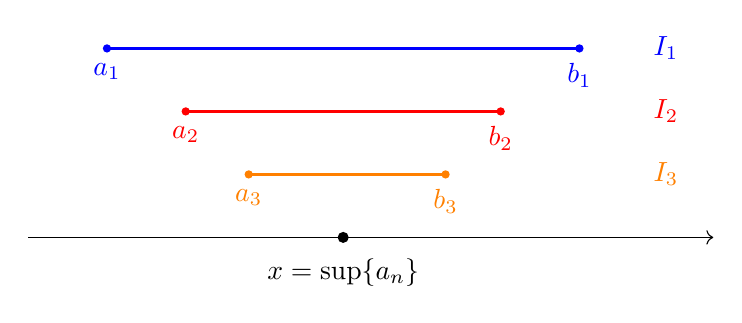
\begin{tikzpicture}[scale=1.0]
    % Number line
    \draw[->] (-0.5,0) -- (8.2,0);

    % I_1 (top)
    \draw[very thick, blue] (0.5,2.4) -- (6.5,2.4);
    \fill[blue] (0.5,2.4) circle (1.5pt) node[below=2pt]{$a_1$};
    \fill[blue] (6.5,2.4) circle (1.5pt) node[below=2pt]{$b_1$};
    \node[blue] at (7.6,2.4) {$I_1$};

    % I_2 (middle)
    \draw[very thick, red] (1.5,1.6) -- (5.5,1.6);
    \fill[red] (1.5,1.6) circle (1.5pt) node[below=2pt]{$a_2$};
    \fill[red] (5.5,1.6) circle (1.5pt) node[below=2pt]{$b_2$};
    \node[red] at (7.6,1.6) {$I_2$};

    % I_3 (bottom)
    \draw[very thick, orange] (2.3,0.8) -- (4.8,0.8);
    \fill[orange] (2.3,0.8) circle (1.5pt) node[below=2pt]{$a_3$};
    \fill[orange] (4.8,0.8) circle (1.5pt) node[below=2pt]{$b_3$};
    \node[orange] at (7.6,0.8) {$I_3$};

    % point x on the number line
    \fill[black] (3.5,0) circle (2pt);
    \node[below=4pt] at (3.5,0) {$x = \sup\{a_n\}$};
  \end{tikzpicture}
  \end{center}

  \note{
    The diagram shows three nested intervals stacked vertically for readability. The blue interval on top is "I" sub 1, with endpoints "a" sub 1 and "b" sub 1. Inside it sits the red "I" sub 2, whose endpoints "a" sub 2 and "b" sub 2 have moved inward. Inside that sits the orange "I" sub 3, tightening further. The black dot on the number line shows the supremum of the left endpoints "a" sub "n", which we proved lies in every interval. One subtlety the theorem leaves implicit: the intersection does not have to be a single point. If the intervals never actually shrink, say all of them equal the same interval, the intersection is that entire interval. Theorem 2.38 only promises nonemptyness. In practice, when the lengths "b" sub "n" minus "a" sub "n" shrink to zero, the intersection collapses to exactly one point, and that is the typical use case. The picture shows the shrinking scenario for visual clarity.
  }
\end{frame}

% =============================================================================
% --- 2.39 Theorem: Nested k-cells ---
% =============================================================================

\begin{frame}{Theorem 2.39: Nested $k$-Cells}
  \begin{thmblock}{Theorem 2.39}
    If $\{I_n\}$ is a sequence of $k$-cells with $I_1 \supset I_2 \supset \cdots$,
    then $\displaystyle\bigcap_{n=1}^\infty I_n \neq \varnothing$.
  \end{thmblock}

  \vspace{0.5em}
  Recall: a \emph{$k$-cell} is a product $[a_1, b_1] \times \cdots \times [a_k, b_k]$.

  \vspace{0.3em}
  \textbf{Strategy:} Apply Theorem 2.38 coordinate-by-coordinate.

  \note{
    A "k"-cell is the Euclidean analog of a closed interval: a product
    of "k" closed intervals, one in each coordinate direction. This
    theorem is the higher-dimensional version of the nested interval
    theorem. The proof is a straightforward reduction: look at each
    coordinate separately and apply the one-dimensional result.
  }
\end{frame}

% --- Proof of 2.39 ---
\begin{frame}{Proof of Theorem 2.39}
  \begin{proofblock}{Proof}
    Let $I_n$ consist of $\mathbf{x} = (x_1, \dots, x_k)$ with $a_{n,j} \leq x_j \leq b_{n,j}$.

    Put $I_{n,j} = [a_{n,j}, b_{n,j}]$. For each fixed $j$:
    \begin{itemize}
      \item $\{I_{n,j}\}_n$ is a nested sequence in $\mathbb{R}^1$.
      \item By Theorem 2.38, some $x_j^* \in I_{n,j}$ for all $n$.
    \end{itemize}
    Setting $\mathbf{x}^* = (x_1^*, \dots, x_k^*)$: $\mathbf{x}^* \in I_n$ for all $n$. \qed
  \end{proofblock}

  \note{
    The proof slices each "k"-cell into its coordinate intervals. "I" sub "n" consists of all points "x" whose "j"-th coordinate "x" sub "j" lies between "a" sub "n" "j" and "b" sub "n" "j", for each "j" from one to "k". So we define "I" sub "n" "j" as the closed interval from "a" sub "n" "j" to "b" sub "n" "j". For each fixed coordinate "j", the sequence of these one-dimensional intervals is nested, because the original "k"-cells are. By Theorem 2.38, each coordinate gives us a real number "x" sub "j" star that lies in "I" sub "n" "j" for every "n". Assembling these coordinates into the vector "x" star gives a point that sits in every "I" sub "n". This reduction works because "k"-cells are products of intervals, and the product of nested intervals is a nested "k"-cell. Not every Euclidean theorem decomposes this cleanly. Compactness on general convex sets, for instance, is much harder. But for axis-aligned boxes, the coordinate-slicing strategy is exactly the right move.
  }
\end{frame}

% =============================================================================
\section{$k$-Cells Are Compact}
% =============================================================================

% =============================================================================
% --- 2.40 Theorem: Every k-cell is compact ---
% =============================================================================

\begin{frame}{Theorem 2.40: Every $k$-Cell Is Compact}
  \begin{thmblock}{Theorem 2.40}
    Every $k$-cell is compact.
  \end{thmblock}

  \vspace{0.5em}
  \textbf{Technique:} Proof by contradiction --- \alert{bisection}.
  \begin{itemize}
    \item Suppose some open cover has no finite subcover.
    \item Repeatedly halve the cell; one half still fails.
    \item The nested halves shrink to a point, which must lie in a single
      cover element --- contradiction.
  \end{itemize}

  \note{
    This is one of the most important theorems of the chapter. Every
    "k"-cell is compact. The technique is bisection, a recurring theme
    in analysis: we assume compactness fails, then repeatedly divide
    the cell into smaller and smaller pieces, always keeping a piece
    where compactness continues to fail. This produces a nested sequence
    shrinking to a point, where a contradiction appears. Let us walk
    through the argument carefully.
  }
\end{frame}

% --- Proof Setup ---
\begin{frame}{Proof of Theorem 2.40 --- Setup}
  \begin{proofblock}{Setup}
    Let $I$ be a $k$-cell with $a_j \leq x_j \leq b_j$. Define the diameter
    \[
      \delta = \left\{\sum_{j=1}^k (b_j - a_j)^2\right\}^{1/2}.
    \]
    Then $\mathbf{x}, \mathbf{y} \in I \Rightarrow |\mathbf{x} - \mathbf{y}| \leq \delta$.
  \end{proofblock}

  \vspace{0.3em}
  \textbf{Assume:} $\{G_\alpha\}$ is an open cover of $I$ with \alert{no finite subcover}.

  \note{
    Let "I" be our "k"-cell, and let delta be its diameter, the Euclidean
    distance from one corner to the opposite corner. Every pair of points
    in "I" has distance at most delta. Suppose for contradiction that some
    open cover of "I" has no finite subcover. Our goal is to derive an
    absurdity from this.
  }
\end{frame}

% --- Proof Step 1: Bisection ---
\begin{frame}{Proof of Theorem 2.40 --- Step 1: Bisection}
  \begin{proofblock}{Halve each coordinate}
    Let $c_j = (a_j + b_j)/2$. The intervals $[a_j, c_j]$ and $[c_j, b_j]$
    determine $2^k$ subcells $Q_1, \dots, Q_{2^k}$ with $\bigcup Q_i = I$.

    \vspace{0.5em}
    If every $Q_i$ had a finite subcover, so would $I$. So at least one
    $Q_i$, call it $I_1$, has \alert{no} finite subcover.
  \end{proofblock}

  \note{
    We halve each coordinate at its midpoint "c" sub "j". Since each of the "k" coordinate intervals splits into two, the whole cell splits into two to the power "k" subcells "Q" sub 1 through "Q" sub 2 to the "k", whose union is all of "I". Now the argument is a pigeonhole on covers: if every one of these finitely many subcells admitted a finite subcover from our bad cover "G" sub alpha, we could glue those finite subcovers together into a finite subcover of the whole "I". That would contradict our assumption that "I" has no finite subcover. So at least one subcell must inherit the failure, and we name it "I" sub 1. The crucial observation is that non-compactness is hereditary: it cannot vanish in all the pieces at once. Since the pieces are smaller, we have made progress toward a contradiction.
  }
\end{frame}

% --- Proof Step 2: Iterate ---
\begin{frame}{Proof of Theorem 2.40 --- Step 2: Iterate}
  \begin{proofblock}{Continue bisecting}
    Subdivide $I_1$ and keep a failing half. Iterate. This yields $\{I_n\}$:
    \begin{enumerate}
      \item[(a)] $I \supset I_1 \supset I_2 \supset \cdots$
      \item[(b)] $I_n$ has no finite subcover from $\{G_\alpha\}$.
      \item[(c)] $\mathbf{x}, \mathbf{y} \in I_n \Rightarrow |\mathbf{x} - \mathbf{y}| \leq 2^{-n} \delta$.
    \end{enumerate}
  \end{proofblock}

  \note{
    We keep bisecting. Inside "I" sub 1 we find a subcell "I" sub 2 with no finite subcover, inside "I" sub 2 we find "I" sub 3, and so on forever. The result is a sequence with three key properties. Part "a": the cells are nested, each inside the previous. Part "b": every "I" sub "n" still defies a finite subcover from the same open cover "G" sub alpha. Part "c": the diameter of "I" sub "n" is at most 2 to the minus "n" times the original diameter delta, because each bisection halves the extent along every coordinate. This geometric shrinkage is the crucial property. A merely linear or polynomial decay would not suffice, because the next step needs the diameter to drop below an arbitrary positive radius after finitely many bisections. Geometric decay achieves this for any radius. The exponential factor 2 to the "n" is doing genuine work here, not just decoration.
  }
\end{frame}

% --- Proof Step 3: The Contradiction ---
\begin{frame}{Proof of Theorem 2.40 --- Step 3: The Contradiction}
  \begin{proofblock}{Reach the contradiction}
    By (a) and Theorem 2.39, some $\mathbf{x}^* \in \bigcap_n I_n$.

    \vspace{0.3em}
    Pick $\alpha$ with $\mathbf{x}^* \in G_\alpha$. Since $G_\alpha$ is open,
    $\exists\, r > 0$: $|\mathbf{y} - \mathbf{x}^*| < r \Rightarrow \mathbf{y} \in G_\alpha$.

    \vspace{0.3em}
    Choose $n$ so large that $2^{-n} \delta < r$. By (c),
    \[
      I_n \subset G_\alpha,
    \]
    a \alert{finite} (single-element) subcover --- contradicting (b). \qed
  \end{proofblock}

  \note{
    By property "a" and Theorem 2.39, the nested "k"-cells share at least one common point "x" star. This point lies in our original cover "G" sub alpha, so some index alpha has "x" star in "G" sub alpha. Since "G" sub alpha is open, there is a radius "r" such that every point within distance "r" of "x" star also lies in "G" sub alpha. Now we use property "c": the diameter of "I" sub "n" is at most 2 to the minus "n" times delta, which we can make smaller than "r" by taking "n" large enough. For such an "n", every point of "I" sub "n" is within "r" of "x" star, so "I" sub "n" fits entirely inside "G" sub alpha. But then "G" sub alpha all by itself is a finite, indeed single-element, subcover of "I" sub "n", which flatly contradicts property "b". That contradiction finishes the proof.
  }
\end{frame}

% --- Diagram: Bisection ---
\begin{frame}{Visualizing the Bisection Argument (for $k = 2$)}
  \vfill
  \begin{center}
  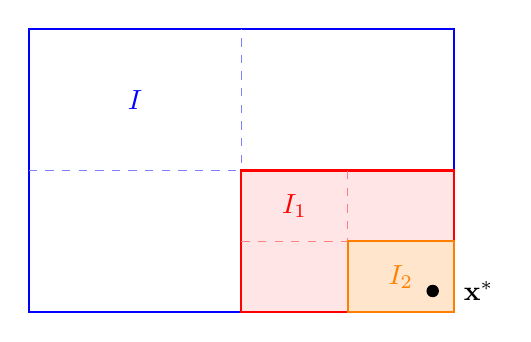
\begin{tikzpicture}[scale=0.9]
    % Outer cell I
    \draw[thick, blue] (0,0) rectangle (6,4);
    \node[blue] at (1.5,3) {$I$};

    % Bisection lines
    \draw[blue!50, dashed] (3,0) -- (3,4);
    \draw[blue!50, dashed] (0,2) -- (6,2);

    % Highlight I_1 (bottom-right quadrant)
    \draw[thick, red, fill=red!10] (3,0) rectangle (6,2);
    \node[red] at (3.75,1.5) {$I_1$};

    % I_2 inside I_1
    \draw[red!50, dashed] (4.5,0) -- (4.5,2);
    \draw[red!50, dashed] (3,1) -- (6,1);
    \draw[thick, orange, fill=orange!20] (4.5,0) rectangle (6,1);
    \node[orange] at (5.25,0.5) {$I_2$};

    \fill[black] (5.7,0.3) circle (2.5pt);
    \node[right] at (6.0,0.3) {$\mathbf{x}^*$};
  \end{tikzpicture}
  \end{center}
  \vfill

  \note{
    Let's visualize the two-dimensional case, where "k" equals two. The big blue rectangle is the original "k"-cell "I". The dashed blue lines split it into four quadrants. The red quadrant, labeled "I" sub 1, is the one we assumed has no finite subcover. Then we bisect again: the red dashed lines split "I" sub 1 into four sub-sub-cells, and the orange rectangle labeled "I" sub 2 is the one that still has no finite subcover. Continuing forever, the nested sequence shrinks geometrically to the single point "x" star in the bottom right. At that point, the cover finally swallows everything around it, terminating the failure, and that contradiction is the whole game. Bisection here is essentially binary search for a failure point. Binary search arguments like this recur throughout analysis, particularly in compactness theorems on function spaces such as Arzela-Ascoli in Chapter 7.
  }
\end{frame}

% =============================================================================
\section{Heine-Borel and Weierstrass}
% =============================================================================

% =============================================================================
% --- 2.41 Theorem: Heine-Borel ---
% =============================================================================

\begin{frame}{Theorem 2.41: Heine-Borel}
  \begin{thmblock}{Theorem 2.41 (Heine-Borel)}
    For a set $E \subset \mathbb{R}^k$, the following are equivalent:
    \begin{enumerate}
      \item[(a)] $E$ is closed and bounded.
      \item[(b)] $E$ is compact.
      \item[(c)] Every infinite subset of $E$ has a limit point in $E$.
    \end{enumerate}
  \end{thmblock}

  \vspace{0.3em}
  \textbf{Note:} The equivalence of (a) and (b) is the classical Heine-Borel theorem.

  \note{
    This is the central structural theorem of the chapter. In Euclidean space,
    three apparently different properties are equivalent. The equivalence of
    "a" and "b", in particular, is the classical Heine-Borel theorem, often
    stated simply as: in Euclidean space, compact means closed and bounded.
    The equivalence of "b" and "c" adds that compactness is also equivalent to
    every infinite subset having a limit point inside the set, a property
    known as the Bolzano-Weierstrass property or limit point compactness.
  }
\end{frame}

% --- Proof Strategy ---
\begin{frame}{Proof Strategy: Theorem 2.41}
  \textbf{Cyclic proof:} (a) $\Rightarrow$ (b) $\Rightarrow$ (c) $\Rightarrow$ (a).

  \vspace{1em}
  \begin{itemize}
    \item (a) $\Rightarrow$ (b): closed + bounded $\subset k$-cell $\Rightarrow$
      closed subset of compact, by Thm 2.40 \& 2.35.
    \item (b) $\Rightarrow$ (c): direct consequence of Theorem 2.37.
    \item (c) $\Rightarrow$ (a): if not bounded or not closed, construct an
      infinite set with no limit point in $E$.
  \end{itemize}

  \note{
    The proof is a three-step cycle. The first direction uses that bounded
    sets fit inside a "k"-cell, which is compact by Theorem 2.40, so a
    closed subset is compact by Theorem 2.35. The second direction follows
    directly from Theorem 2.37, which we just proved. The third direction
    is the only one that requires work: we must show that if property "c"
    holds, the set is forced to be both bounded and closed.
  }
\end{frame}

% --- Proof (a) implies (b) ---
\begin{frame}{Proof --- (a) $\Rightarrow$ (b)}
  \begin{proofblock}{Closed + bounded $\Rightarrow$ compact}
    \begin{itemize}
      \item $E$ bounded $\Rightarrow$ $E \subset I$ for some $k$-cell $I$.
      \item $I$ is compact (Theorem 2.40).
      \item $E$ is closed, so $E$ is a closed subset of the compact set $I$.
      \item By Theorem 2.35, $E$ is compact. \qed
    \end{itemize}
  \end{proofblock}

  \note{
    Assume "E" is closed and bounded. Boundedness means "E" sits inside some "k"-cell "I". Theorem 2.40, the hardest result we proved, tells us this "k"-cell is compact. Since "E" is also closed, it is a closed subset of the compact set "I", and by Theorem 2.35, closed subsets of compact sets are compact. Therefore "E" is compact. This direction is purely a packaging step, no new ideas. The hard work is already done elsewhere; this slide just wires the components.
  }
\end{frame}

% --- Proof (b) implies (c) ---
\begin{frame}{Proof --- (b) $\Rightarrow$ (c)}
  \begin{proofblock}{Compact $\Rightarrow$ every infinite subset has a limit point in $E$}
    This is exactly Theorem 2.37. \qed
  \end{proofblock}

  \note{
    This direction is immediate. Theorem 2.37 says precisely that in a
    compact set, every infinite subset has a limit point inside the set.
    Nothing more to prove.
  }
\end{frame}

% --- Proof (c) implies (a) Step 1 ---
\begin{frame}{Proof --- (c) $\Rightarrow$ (a): $E$ is bounded}
  \begin{proofblock}{If $E$ is unbounded, (c) fails}
    Suppose $E$ is not bounded. Choose $\mathbf{x}_n \in E$ with $|\mathbf{x}_n| > n$.
    \begin{itemize}
      \item $S = \{\mathbf{x}_n\}$ is infinite.
      \item Any $\mathbf{y} \in \mathbb{R}^k$: only finitely many $\mathbf{x}_n$ satisfy
        $|\mathbf{x}_n - \mathbf{y}| < 1$ (since $|\mathbf{x}_n| > n$).
      \item So $S$ has no limit point in $\mathbb{R}^k$, hence none in $E$.
      \item Contradicts (c). Therefore $E$ is bounded.
    \end{itemize}
  \end{proofblock}

  \note{
    This is the direction where the proof earns its keep: property "c" has to force both boundedness and closedness of "E". We start with boundedness. Suppose for contradiction that "E" is not bounded. Then we can pick a sequence of points "x" sub "n" in "E" with norms growing beyond "n". Call this infinite set "S". Now take any candidate limit point "y" in Euclidean space. The triangle inequality shows that if "x" sub "n" has norm greater than "n", then for "n" larger than the norm of "y" plus one, the distance from "x" sub "n" to "y" is already bigger than one. So only finitely many "x" sub "n" lie within distance one of "y". That means "y" cannot be a limit point of "S". Since "y" was arbitrary, "S" has no limit point anywhere in Euclidean space, let alone inside "E". Property "c" forbids that, so "E" must have been bounded after all.
  }
\end{frame}

% --- Proof (c) implies (a) Step 2 Setup ---
\begin{frame}{Proof --- (c) $\Rightarrow$ (a): $E$ is closed (setup)}
  \begin{proofblock}{Suppose $E$ is not closed}
    Let $\mathbf{x}_0$ be a limit point of $E$ with $\mathbf{x}_0 \notin E$.

    For each $n$, choose $\mathbf{x}_n \in E$ with $|\mathbf{x}_n - \mathbf{x}_0| < 1/n$.
    Let $S = \{\mathbf{x}_n\}$.
    \begin{itemize}
      \item $S$ is infinite (otherwise $|\mathbf{x}_n - \mathbf{x}_0|$ has a positive
        lower bound, contradiction).
      \item $\mathbf{x}_0$ is a limit point of $S$.
    \end{itemize}
  \end{proofblock}

  \note{
    Now we handle closedness. Suppose "E" is not closed. Then by definition, there is some limit point "x" naught of "E" that does not belong to "E". Since "x" naught is a limit point, we can find points "x" sub "n" of "E" inside arbitrarily small balls around "x" naught. Specifically, for each "n" we pick some "x" sub "n" in "E" within distance one over "n" of "x" naught. Call the collection "S". "S" must be infinite, because if it were finite the distances from its points to "x" naught would have a positive minimum, which our one-over-"n" bound will eventually violate. Moreover, because the "x" sub "n" get arbitrarily close to "x" naught, "x" naught is a limit point of "S". The strategic point of this setup is to concentrate all the potential limit points onto the single candidate "x" naught, so that on the next slide we can rule out every alternative limit point one by one.
  }
\end{frame}

% --- Proof (c) implies (a) Step 3 Finish ---
\begin{frame}{Proof --- (c) $\Rightarrow$ (a): $E$ is closed (finish)}
  \begin{proofblock}{$S$ has no other limit point in $\mathbb{R}^k$}
    For $\mathbf{y} \neq \mathbf{x}_0$, by the triangle inequality:
    \[
      |\mathbf{x}_n - \mathbf{y}| \geq |\mathbf{x}_0 - \mathbf{y}| - \tfrac{1}{n} \geq \tfrac{1}{2} |\mathbf{x}_0 - \mathbf{y}|
    \]
    for large $n$. So $\mathbf{y}$ is not a limit point of $S$ (Thm 2.20).

    \vspace{0.3em}
    $S \subset E$, infinite, but its only limit point $\mathbf{x}_0 \notin E$.
    This contradicts (c). \qed
  \end{proofblock}

  \note{
    We claim "x" naught is the only possible limit point of "S" in Euclidean space. Take any other point "y" distinct from "x" naught. By the reverse triangle inequality, the distance from "x" sub "n" to "y" is at least the distance from "x" naught to "y" minus the distance from "x" sub "n" to "x" naught, which is at most one over "n". For "n" large enough, that shrinking correction is smaller than half the distance from "x" naught to "y", so we get the lower bound shown on the slide: at least half the distance from "x" naught to "y", a fixed positive constant. This means a small enough neighborhood of "y" contains at most finitely many "x" sub "n", so by Theorem 2.20, "y" is not a limit point of "S". Since only "x" naught could be a limit point of "S", and "x" naught is not in "E", the infinite subset "S" of "E" has no limit point in "E". That contradicts property "c". Therefore "E" must be closed, completing the entire Heine-Borel proof.
  }
\end{frame}

% --- Diagram: Closure argument ---
\begin{frame}{Visualizing the Closure Argument}
  \vfill
  \begin{center}
  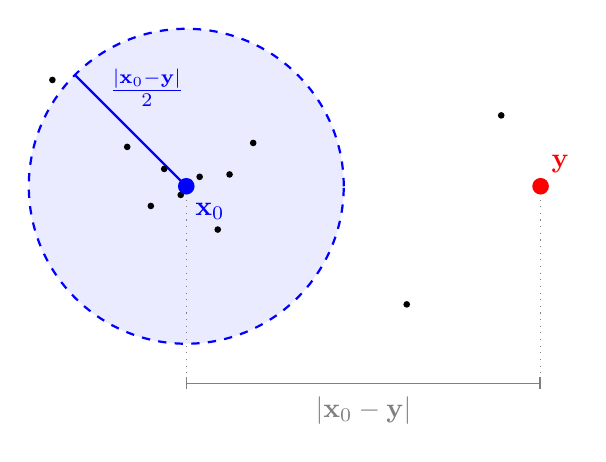
\begin{tikzpicture}[scale=1.0]
    % Ball around x_0 with radius |x_0 - y|/2 = 2
    \fill[blue!8] (0,0) circle (2);
    \draw[thick, blue, dashed] (0,0) circle (2);

    % Radius marker inside the ball
    \draw[blue, thick] (0,0) -- ({2*cos(135)}, {2*sin(135)});
    \node[blue] at (-0.5, 1.25) {$\tfrac{|\mathbf{x}_0 - \mathbf{y}|}{2}$};

    % Distance indicator below
    \draw[gray, dotted] (0,0) -- (0,-2.5);
    \draw[gray, dotted] (4.5,0) -- (4.5,-2.5);
    \draw[gray, |-|] (0,-2.5) -- (4.5,-2.5);
    \node[gray, below] at (2.25, -2.55) {$|\mathbf{x}_0 - \mathbf{y}|$};

    % Sequence points x_n converging to x_0 (inside the ball)
    \fill[black] (0.85, 0.55) circle (1.2pt);
    \fill[black] (-0.75, 0.5) circle (1.2pt);
    \fill[black] (0.4, -0.55) circle (1.2pt);
    \fill[black] (-0.28, 0.22) circle (1.2pt);
    \fill[black] (0.17, 0.12) circle (1.2pt);
    \fill[black] (-0.07, -0.11) circle (1.2pt);
    \fill[black] (0.04, 0.05) circle (1.2pt);
    \fill[black] (-0.45, -0.25) circle (1.2pt);
    \fill[black] (0.55, 0.15) circle (1.2pt);

    % A few x_n outside the ball (finitely many)
    \fill[black] (-1.7, 1.35) circle (1.2pt);
    \fill[black] (4.0, 0.9) circle (1.2pt);
    \fill[black] (2.8, -1.5) circle (1.2pt);

    % x_0
    \fill[blue] (0,0) circle (3pt);
    \node[blue] at (0.3, -0.32) {$\mathbf{x}_0$};

    % y
    \fill[red] (4.5,0) circle (3pt);
    \node[red] at (4.75, 0.28) {$\mathbf{y}$};
  \end{tikzpicture}
  \end{center}

  \begin{center}
    \small All but finitely many $\mathbf{x}_n$ lie inside the ball --- so $\mathbf{y}$ is not a limit point of $S$.
  \end{center}
  \vfill

  \note{
    Let's visualize the idea. "x" naught is the limit point of "S" that is not in "E", and we want to rule out every other point "y" as a limit point. Draw a ball around "x" naught with radius equal to half the distance from "x" naught to "y". Because the "x" sub "n" get arbitrarily close to "x" naught, eventually all of them fall inside this ball, leaving only finitely many outside. The point "y" sits at twice that radius from "x" naught, safely outside the ball. So a neighborhood of "y" with the same radius can contain at most finitely many of the "x" sub "n", which means by Theorem 2.20 that "y" cannot be a limit point of "S". Only "x" naught qualifies.
  }
\end{frame}

% --- Remark on 2.41 ---
\begin{frame}{Remark on Theorem 2.41}
  \begin{remblock}{Scope of Heine-Borel}
    \begin{itemize}
      \item (b) $\iff$ (c) holds in \emph{any} metric space (Exercise 26).
      \item (a) $\Rightarrow$ (b) is \alert{special to $\mathbb{R}^k$}.
      \item Counterexamples: $\mathscr{L}^2$ (Chap.~11), Exercise 16.
    \end{itemize}
  \end{remblock}

  \note{
    One important caveat. The equivalence of "b" and "c" holds in every metric
    space, a result developed in Exercise 26. However, the equivalence of
    "a" with "b" and "c" is special to Euclidean space. In general metric
    spaces, closed and bounded does not imply compact. For instance, the
    space "L" squared discussed in Chapter 11 provides a counterexample,
    and so does Exercise 16. So the Heine-Borel theorem in its most
    familiar form is genuinely a theorem about Euclidean geometry.
  }
\end{frame}

% =============================================================================
% --- 2.42 Theorem: Weierstrass ---
% =============================================================================

\begin{frame}{Theorem 2.42 (Weierstrass)}
  \begin{thmblock}{Theorem 2.42 (Bolzano-Weierstrass)}
    Every bounded infinite subset of $\mathbb{R}^k$ has a limit point in $\mathbb{R}^k$.
  \end{thmblock}

  \vspace{0.5em}
  \begin{proofblock}{Proof}
    \begin{itemize}
      \item $E$ bounded $\Rightarrow$ $E \subset I$ for some $k$-cell $I$.
      \item $I$ compact (Theorem 2.40).
      \item $E$ infinite subset of compact $I$ $\Rightarrow$ $E$ has a limit
        point in $I$ (Theorem 2.37). \qed
    \end{itemize}
  \end{proofblock}

  \note{
    We close with the classical Bolzano-Weierstrass theorem. Every bounded
    infinite subset of Euclidean space has a limit point. The proof is a
    one-line synthesis of our main results. A bounded set sits in a
    "k"-cell, which is compact by Theorem 2.40. An infinite subset of a
    compact set has a limit point in the compact set by Theorem 2.37.
    So our bounded infinite "E" has a limit point, somewhere in the
    enclosing "k"-cell.
  }
\end{frame}

% =============================================================================
% --- Summary ---
% =============================================================================

% --- Build 1/5 ---
\begin{frame}{Summary}
  \textbf{Key takeaways from this section:}
  \begin{itemize}
    \item A set is \alert{compact} if every open cover has a finite
      subcover (Def.\ 2.32).
  \end{itemize}

  \note{
    Let us summarize the main ideas. We introduced compactness as the
    property that every open cover admits a finite subcover. This is a
    finiteness condition on the set, and it is the organizing concept of
    the whole section.
  }
\end{frame}

% --- Build 2/5 ---
\begin{frame}{Summary}
  \textbf{Key takeaways from this section:}
  \begin{itemize}
    \item A set is \alert{compact} if every open cover has a finite
      subcover (Def.\ 2.32).
    \item Compactness is \emph{intrinsic}: independent of ambient space
      (Thm.\ 2.33). Compact sets are closed (Thm.\ 2.34), and closed
      subsets of compact sets are compact (Thm.\ 2.35).
  \end{itemize}

  \note{
    We proved that compactness is intrinsic to the set and does not
    depend on how we embed it. We established two basic preservation
    theorems: compact sets are always closed, and closed subsets of
    compact sets are compact.
  }
\end{frame}

% --- Build 3/5 ---
\begin{frame}{Summary}
  \textbf{Key takeaways from this section:}
  \begin{itemize}
    \item A set is \alert{compact} if every open cover has a finite
      subcover (Def.\ 2.32).
    \item Compactness is \emph{intrinsic}: independent of ambient space
      (Thm.\ 2.33). Compact sets are closed (Thm.\ 2.34), and closed
      subsets of compact sets are compact (Thm.\ 2.35).
    \item \alert{Finite intersection property}: a collection of compact sets
      with nonempty finite intersections has nonempty total intersection
      (Thm.\ 2.36). Infinite subsets of compact sets have limit points
      in the set (Thm.\ 2.37).
  \end{itemize}

  \note{
    The finite intersection property tells us that nested or mutually
    intersecting compact sets cooperate at infinity. Infinite subsets
    of compact sets always have a limit point within the compact set,
    which is the germ of sequential compactness.
  }
\end{frame}

% --- Build 4/5 ---
\begin{frame}{Summary}
  \textbf{Key takeaways from this section:}
  \begin{itemize}
    \item Every $k$-cell is compact (Thm.\ 2.40) via \alert{bisection} and
      nested $k$-cells (Thms.\ 2.38, 2.39). \alert{Heine-Borel}
      (Thm.\ 2.41): in $\mathbb{R}^k$, closed and bounded $\iff$ compact
      $\iff$ every infinite subset has a limit point in the set.
  \end{itemize}

  \note{
    The hardest theorem is that every "k"-cell is compact, proved by
    bisection using the nested "k"-cell theorem. This feeds into the
    Heine-Borel theorem, which says that in Euclidean space, three
    apparently different properties coincide: closed and bounded,
    compact, and having the property that every infinite subset has
    a limit point in the set.
  }
\end{frame}

% --- Build 5/5 ---
\begin{frame}{Summary}
  \textbf{Key takeaways from this section:}
  \begin{itemize}
    \item Every $k$-cell is compact (Thm.\ 2.40) via \alert{bisection} and
      nested $k$-cells (Thms.\ 2.38, 2.39). \alert{Heine-Borel}
      (Thm.\ 2.41): in $\mathbb{R}^k$, closed and bounded $\iff$ compact
      $\iff$ every infinite subset has a limit point in the set.
    \item \alert{Bolzano-Weierstrass} (Thm.\ 2.42): every bounded infinite
      subset of $\mathbb{R}^k$ has a limit point.
  \end{itemize}

  \vspace{0.5em}
  \textbf{Coming up next:} Perfect sets and the Cantor set.

  \note{
    We closed with the Bolzano-Weierstrass theorem as a direct corollary. In the next section we will study perfect sets, which are closed sets in which every point is a limit point. We will also meet the Cantor set, one of the most remarkable examples in all of analysis. See you there!
  }
\end{frame}

\end{document}
